\documentclass{llncs}

\usepackage[utf8x]{inputenc}
\usepackage{amssymb}
\usepackage{amsmath}
\usepackage{graphicx}
\usepackage{multicol} 
 \usepackage[spanish]{babel} % espanol, ingles



% \documentclass{article}
%opening
\title{De la Universidad a la industria del software y viceversa: Una experiencia centrada en la aplicación de nuevas tecnologías, adoptadas por la industria, a proyectos finales de asignaturas}

\author{Marcela Daniele, Marcelo Uva, Ariel Arsaute y Franco Brusatti }

\institute{Departamento de Computaci\'on, FCEFQyN, Universidad Nacional de R\'{\i}o Cuarto, R\'{\i}o Cuarto, Argentina. 
Email: \email{$\{$marcela,uva,fbrusatti,aarsaute$\}$@dc.exa.unrc.edu.ar}
}

\begin{document}

 

\maketitle


\begin{abstract}
Durante la última década, la relación Universidad e Industria de desarrollo de software se ha vuelto cada vez más estrecha. Pequeñas, medianas y grandes empresas se acercan continuamente a las universidades en busca de recursos humanos calificados. El crecimiento y expansión del mercado informático ha propiciado, la generación y adopción de nuevas 
metodologías de desarrollo, nuevas modalidades de trabajo por ejemplo  desarrollos outsourcing.
Junto con éstas, han surgido nuevas tecnologías que brindan el soporte necesario para las actividades de administración, 
gestión, planificación, implementación, diseño, testing  y control en  la producción 
del software. 
En este trabajo se presenta una experiencia desarrollada durante los años 2014 y 2015 dentro de las asignaturas Análisis 
y Diseño de Sistemas. La propuesta consiste en el desarrollo de un proyecto-taller integrador que aplica un 
set de herramientas y tecnologías utilizadas en la industria del desarrollo de software actual, estableciendo un puente más 
directo entre formación académica y necesidad del mercado.

\end{abstract}


\begin{multicols}{2} 



\section{Introducción}
Durante la última década, la relación Universidad e Industria de desarrollo de software se ha vuelto cada vez más estrecha. Pequeñas, medianas y grandes empresas se acercan continuamente a las universidades en busca de analistas, programadores, ingenieros de software, etc.
El constante crecimiento y expansión del mercado informático, en todos los ámbitos, hace cada vez más visible la necesidad de contar con 
recursos humanos calificados. Paralelamente, dicho crecimiento ha propiciado en la industria, la generación y adopción de nuevas 
metodologías de desarrollo y conjuntamente, nuevas modalidades de trabajo por ej. desarrollos outsourcing.
Nuevas tecnologías han surgido con el objeto de dar el soporte necesario para las actividades de administración, 
gestión, planificación, implementación, diseño, automatización del testing, seguimiento y control de las tareas que hacen a la producción 
del software. Muchas de estas tecnologías poco a poco han ido  incorporándose en las currículas de las carreras de informática. De esta manera se ha establecido una relación de necesidad entre Universidad e Indrustria de desarrollo de sofware en ambos sentidos.
En el marco de los proyectos PIIMEG CITA (Proyectos de Investigación e Innovación para el Mejoramiento de la Enseñanza de Grado) pertenecientes a la Universidad Nacional de Río Cuarto se han llevado adelante una serie de propuestas en pos de detectar, analizar y ejecutar acciones concretas con el fin de realizar aportes para solucionar problemáticas observadas en las asignaturas de 3er. año de las carreras de Analista, Profesorado y Licenciatura en Ciencias de la Computación. 
En este trabajo se presenta una experiencia desarrollada durante los años 2014 y 2015 dentro de las asignaturas Análisis y Diseño de Sistemas. 
La propuesta consiste en el desarrollo de un proyecto-taller en donde, además de integrar los contenidos teórico-prácticos abordados en las 
asignaturas de tercer año, se incorporen un conjunto de tecnologías utilizadas en la industria del desarrollo de software actual. 
El resto del trabajo está organizado de la siguiente manera: en la sección 2 se presentan los fundamentos de la propuesta y se plantean los 
objetivos. La sección 3 presenta la metodología de desarrollo aplicada. En la sección 4 se presenta la propuesta, planificación, 
tecnologías y herramientas utlizadas. En la sección 5 se realiza una evalución de la propuesta, y finalmente, las conclusiones.

\section{Fundamentos}\label{fundamenta}
La planificación y ejecución de procesos de enseñanza-aprendizaje para cursos de ingeniería de software (IS), plantean un gran desafío a los docentes universitarios involucrados. La necesidad de una actualización dinámica de los contenidos no debe provocar el descuido de conceptos básicos vinculados a los principios fundamentales del desarrollo de sistemas de software.
El cuerpo docente, autor de este artículo, tiene a cargo el dictado de los cursos Análisis y Diseño de Sistemas e Ingeniería de Software, durante el tercer año de las carreras: Licenciatura y Profesorado en Ciencias de la Computación y Analista en Computación, de la Universidad Nacional de Río Cuarto.

Los conceptos básicos de IS, son introducidos en el curso de Análisis y Diseño de Sistemas. En este se presentan diferentes metodologías de desarrollo de software [ver$$$$]. 

Para el curso de Ingeniería de Software, el principal propósito es que el alumno tome conocimiento de los conceptos más avanzados de IS; desde la planificación y gestión del proyecto hasta técnicas de testing o prueba. Al mismo tiempo se cubren  conceptos transversales a las etapas de desarrollo como el gerenciamiento de la configuración de software



Esta metodología incorpora la realización de proyectos-taller, abordando específicamente el desafío de la utilización de herramientas que asistan en las actividades de gestión de proyectos de software [ver$$$$] y ayuden al mismo tiempo la compresión profunda de los temas abordados. 
El principal propósito es conseguir que los alumnos vivencien situaciones muy cercanas a la realidad y, de esta manera, disminuir la brecha entre la teoría universitaria y la realidad profesional.



El dictado de la asignatura IS se divide en clases teóricas, clases prácticas y proyectos-taller

Durante los años 2014 y 2015, se abordó importantes desafíos a cubrir en la enseñanza de ingeniería de software, introduciendo la utilización de herramientas que permitan automatizar la gestión de proyectos de software [Ver$$$$]. 

En este marco, se logró fomentar el uso de una metodología de desarrollo de software en proyectos reales. Promoviendo de esta manera la división de roles operativos y gerenciales entre los integrantes de un grupo de desarrollo de software, capacitándolos para la evaluación y selección de diferentes herramientas aplicables a las actividades de gestión de software.

En el año 2014, se presentó ……

En el año 2015, se presentó ……


\section{Metodología de desarrollo aplicada al proyecto integrador} \label{metodologia}
% \section{Metodologías Tradicionales y Metodologías Ágiles}\label{metodologia}
En el marco de las asignaturas de Ingeniería de Sofware, se presenta una visión general sobre las diferentes metodologías utilizadas en 
el de desarrollo de 
software\cite{pressman,jalote}.
Algunos de los ciclos de vida del software estudiados son:  el lineal o secuencial, el método del Análisis Estructurado de Yourdon\cite{yourdon}, 
desarrollo basado en componentes, diseño por contratos\cite{meyer} de Bertrand Meyer, entre otros. 
Particularmente, se pone énfasis en el Proceso Unificado\cite{pu}, como método de desarrollo
orientado a objetos tradicional  y en Scrum\cite{agile}, como metodología de desarrollo ágil.\\ 
En este trabajo se presenta una modificación al proyecto de articulación de contenidos mencionado en la sección
\ref{fundamenta} meditante la 
incorporación de un 
conjunto  de herramientas 
que la industria de desarrollo de software utiliza intensamente en la actualidad. Dichas tecnologías están intimamente ligadas a la 
aplicación de 
metodologías ágiles\cite{metagiles}, especialmente con Scrum, metodología seleccionada por el equipo docente para el desarrollo de este 
proyecto integrador.
Scrum es una metodología ágil que posibilita trabajar en ambientes muy cambiantes, permitiendo replanteamientos continuos. 
Por otro lado, reduce el tiempo de producción y de comercialización del producto, aporta un gran beneficio o 
valor agregado al cliente, minimiza los riesgos de desperdiciar esfuerzo/tiempo en la construcción de artefactos que no serán utilizados 
o que no son fundamentales para el cliente. Facilita también la comunicación entre todos los integrantes del proyecto. 
La documentación producida dentro de un proyecto Srum es relativa al usuario, dueño, producto y equipo.  Scrum es un marco de 
trabajo basado sobre la premisa de que el equipo de desarrollo conocerá la mejor manera de resolver el problema que se le presenta. 
La reunión de planificación de cada conjunto de requerimientos a producir se describe en términos del resultado deseado, 
en lugar de un conjunto de criterios de ingreso, definiciones y tareas. 
Scrum se basa en una auto-organización, con un equipo multifuncional y sin líder (dentro del equipo). 
El equipo es apoyado por dos individuos quienes ocupan los roles de Scrum Master y  Product Owner. 
El Scrum Master es una especie de entrenador para el equipo, su función es ayudar a los miembros del mismo a utilizar el marco que ofrece 
la metodología para conseguir un alto nivel de productividad. Mientras que el Product Owner representa los negocios, clientes o 
usuarios. Éste, guía al equipo hacia la construcción del producto esperado.
 Los proyectos Scrum avanzan en orden a la definición de los sprints, que son las iteraciones que poseen una duración de entre dos y cuatro semanas. 
En el inicio de cada sprint, los miembros del equipo se comprometen a producir un cierto número de características que se enumeran en 
el artefacto conocido como Product Backlog del proyecto.  Al final de cada sprint, cada funcionalidad (conocida como user story) debe estar 
codificada,
 probada e integrada a una versión demo del sprint anterior. Luego se realiza una revisión, y por último se presenta la nueva funcionalidad
 frente al Product Owner y las otras partes interesadas que proporcionarán información requerida para el siguiente sprint. 
Las iteraciones han de continuar hasta obtener el producto deseado.
Como se puede observar de lo expuesto, Scrum establece una forma de trabajo en donde todo el equipo se auto-regula y en donde no hay 
una documentación establecida a priori. Cada equipo utilizará los elementos que le sean necesarios para poder llevar adelante el conjunto de 
user stories
con el cual se ha comprometido. Algunos equipos podrán utilizar diagramas UML\cite{uml}, otros utilizarán diagramas de flujos de datos, etc.
En la figura \ref{figu1} se esquematiza todo el proceso.
\section{Descripción de la propuesta} \label{propuesta}

La propuesta presentada en este trabajo consiste 
en el desarrollo de un proyecto integrador donde, además de integrar los contenidos teórico-prácticos 
estudiados en las asignaturas de Ingeniería de Sofware, se incorpore un conjunto de tecnologías y herramientas utilizadas en la industria del 
desarrollo de software actual,
permitiendo
establecer un vínculo estrecho entre el futuro egresado y las empresas de desarrollo de software. \\
\subsection{Objetivos}
A continuación se enumeran los objetivos de esta propuesta:
 \begin{itemize}
 \item Integrar en un  proyecto de desarrollo de software los contenidos trabajados en tercer año, fundamentalmente, aquellos
 pertenecientes a las asignaturas de Ingeniería de Sofware. 
 \item Aplicar una metodología de desarrollo ágil como Scrum. Aprovechando de esta manera los beneficios que conlleva la misma y a sabiendas de que 
 es una de la más utilizadas por las empresas de desarrolo de software.
 \item Simular un ambiente de trabajo con características similares a las de un ambiente de trabajo real. Para ello se establecen objetivos grupales 
 y es el mismo grupo quien se auto-gestiona. Si bien los objetivos son grupales, en el marco del proyecto integrador, 
 se realiza un seguimiento y valoración particular de cada uno de los 
 estudiantes, su integración con el resto, su compromiso, su forma de trabajo, etc.
 \item Desarrollar en los estudiantes habilidades para adoptar y obtener beneficios  de un conjunto de herramientas utilizadas en la industria del software. 
 El objetivo no es sólo que aprendan a usar una herramienta, 
%  \newpage
 sino que sean capaces de seleccionar las herramientas adecuadas en futuros proyectos.
 
 
 \subsection{Organización y planificación}
El poyecto integrador es planificado para ejecutarse durante el primer cuatrimestre del año. Cabe señalar
que dentro del equipo docente de la asignatura, se ha seleccionado a un docente  con dedicación part-time para la coordinación general 
del poyecto integrador. La selección de este docente fue motivada por la vinculación que  el mismo posee con la industria de desarrollo de software. 
Este docente es fundador de una empresa de desarrollo de software local y está habituado a formar parte de equipos de trabajo
con desarrolladores a nivel internacional en proyectos bajo la modalidad outsorcing y freelance. 
Uno de los objetivos del proyecto integrador es la aplicación de una metodología ágil, es por ello que el proyecto está guiado por Srum.
En cada una de las fases del ciclo de vida, se aplica una herramienta específica. No es objetivo de este 
proyecto agregar complejidad en demasia  ni sobrecargar tiempos de desarrollo. Sino que se focaliza en que cada 
grupo de estudiantes pueda completar el trabajo, usando las tecnologías propuestas.  
 
 \end{itemize}
% 
%  \end{multicols}
%   \begin{figure}[b!]
%    \centering
% 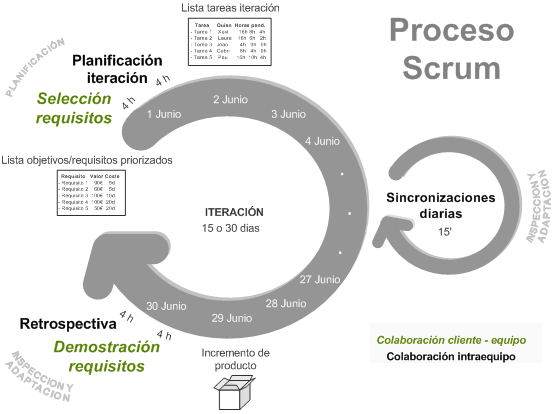
\includegraphics[width=0.9 \textwidth]{f2}
%     \caption{Proceso de desarrollo Scrum}
%     \label{figu1}
%   \end{figure}
%  \begin{multicols}{2} 

% \subsection{Organización y planificación}
% El poyecto integrador es planificado para ejecutarse durante el primer cuatrimestre del año. Cabe señalar
% que dentro del equipo docnete de la asignatura, se ha seleccionado a un docente  con dedicación part-time para la coordinación general 
% del poyecto integrador. La selección de este docente fue motivada por la vinculación que  el mismo posee con la industria de desarrollo de software. 
% Este docente es fundador de una empresa de desarrollo de software local y está habituado a formar parte de equipos de trabajo
% con desarrolladores a nivel internacional en proyectos bajo la modalidad outsorcing y freelance.
% 
% Uno de los objetivos del proyecto integrador es la aplicación de una metodología ágil, es por ello que el proyecto está guiado por Srum.
% En cada una de las fases del ciclo de vida, se aplica una herramienta específica. No es objetivo de este 
% proyecto complejizar ni sobrecargar tiempos de desarrollo. Sino que se focaliza en que cada 
% grupo de estudiantes pueda completar el trabajo, usando las tecnologías propuestas.  
Se formaron equipos de tres estudiantes, más el Scrum Master\cite{agile}, rol ocupado por un docente de la asignatura.\\
El proyecto desarrollado en el año 2014 consistió en la construcción de un  sistema web en donde un usuario  pueda loguearse y publicar avisos de compra
 y venta de vehículos. En el año 2015, el proyecto desarrollado fue la construcción de una vesión del juego \textit{Cuatro en línea}. 
 El diseño del problema se planteó de una manera simplificada evitando el crecimiento del proyecto de manera descontrolada.
 El equipo docente estableció un Product Backlog inicial, y en la medida de que cada grupo avanzaba se incluían 
 nuevas funcionalidades. Todos los grupos asistían a un encuentro semanal de dos horas donde se introducían las herramientas y se establecían los 
 objetivos según la planificación correspondiente. Durante uno de los encuentros, los ayudantes alumno, con los que cuentan las asignaturas
 involucradas en este trabajo, elaboraron un taller sobre una de las herramientas seleccionadas. Esto permitió realizar aportes a su formación docente, 
 y al mismo tiempo brindó  una mirada diferente al aprovechamiento de estas tecnologías.
 En el resto de los encuentros, los docentes realizaron el seguimiento de cada grupo de estudiantes.
 A continuación se presenta, a modo de ejemplo, la planificación para el proyecto integrador
llevado a cabo durante el año 2014.

\begin{itemize}
 \item Marzo 18 - Presentación general del taller e introducción de Git.
\item Abril 1 - SCRUM y Definnición del SRS (Sofware Requeriment Specification). PivotalTracker - Creación del Product Backlog.
\item Abril 8 - Introducción a Java - Eclipse / ActiveJDBC / Postgresql.
\item Abril 15 - Taller de  Maven y JUnit.
\item Abril 22 - Diseño / Implementación.
\item Abril 29 - Diseño / Implementación.
\item Mayo 6 - Taller de JUnit - definición de la Test Suite.
\item Mayo 13 - Diseño / Implementación.
\item Mayo 20 - Checkpoint (Test Suite running).
\item Mayo 27 - Taller Spark - Sinatra e incorporación de la capa web.
\item Junio 3 - Implementación 
\item Junio 10 - Implementación
\item Junio 17 - Presentación de grupos
\end{itemize}

\subsection{Tecnologías y herramientas utilizadas}
La industria del software se encuentra en continua expansión. Esto requiere la incorporación de nuevas tecnologías para generar
nuevas tecnologías. Sólo incorporando nuevas herramientas de soporte para estos procesos es que se logra producir sistemas para millones
de usuarios, como por ejemplo las redes sociales. \\
Las herramientas utilizadas en este proyecto fueron las siguientes:
 \begin{itemize}
 \item Github\cite{github}: plataforma de desarrollo colaborativo de software para alojar proyectos utilizando el sistema de control de versiones Git. El código se almacena de forma pública, aunque también se puede hacer de forma privada, creando una cuenta de pago. 
 \item Git\cite{git}: sistema de control de versiones distribuido, libre y gratuito.
 \item Java 8\cite{java8}: lenguaje de programación informática de propósito general que es concurrente, basado en clases y orientado a objetos.
 \item Postgresql\cite{postgresql}: sistema de base de datos objeto-relacional con características de los sistemas de base de datos propietarios tradicionales con mejoras de los sistemas de base de datos de la nueva generación.
 \item ActiveJDBC\cite{activejdbc}: ORM (Object Relational Mapping) para desarrollo ágil. Es una implementación en el lenguaje Java del patrón arquitectural Active Record.
 \item JUnit\cite{junit}: framework para escribir tests (pruebas de software). Es una implementación de la arquitectura xUnix para unit testing.
 \item Spark\cite{spark}: framework inspirado en Sinatra para crear aplicaciones web con Java 8.
 \item Sinatra\cite{sinatra}: framework para aplicaciones web de software libre y código abierto con una DSL (Domain Specific Language) escrito en Ruby on Rail.
 \item PivotalTracker\cite{pivotaltracker}: herramienta para la gestión de proyectos ágiles.
%  \item SCRUM [23]: metodología ágil para desarrollar proyectos de software.
 \item Maven\cite{maven}: herramienta de software para la gestión y construcción de proyectos Java creada por Jason van Zyl, de Sonatype, en 2002. Es similar en funcionalidad a Apache Ant (y en menor medida a PEAR de PHP y CPAN de Perl), con un modelo de configuración de construcción más simple, basado en un formato XML.
 \item GanttProject\cite{gantproject}: herramienta para crear una completa planificación de un proyecto de forma visual. Todo queda bajo control en GanttProject, desde los recursos necesarios en forma de personal, los días festivos, hasta dividir el proyecto en un árbol de tareas y asignar a cada uno los recursos oportunos.
\end{itemize}












\section{Resultados}\label{resultado}

\end{multicols}


\fbox{
\begin{minipage}[b][1\height]%
[t]{1\textwidth} 


\textbf{Encuesta de finalización de cuatrimetre 3er. año} \\ 
1. ¿Cúales fueron las materias que cursaste en este cuatrimestre ?\\
2. ¿Cuáles regularizaste?\\
3. ¿Te pareció interesante la propuesta del taller?\\
      Si   -  No - Parcilmente . Justifique en cada caso.\\
4. ¿Cúantas horas semanales promedio le dedicaste al taller?\\
5. ¿Se comprendió  el objetivo del taller al momento de presentarlo? 
      Si   -  No - Parcilmente \\
6. ¿Habías realizado algún proyecto de materia utilizando alguna metodología de desarrollo? Si(Cuál) - No\\
7. ¿ Todos los integrantes del grupo trabajaron de igual manera? Si – No – En ocasiones\\
8. Que porcentaje del total aportaste al proyecto.\\
9. En general, como calificas la experiencia de trabajo grupal. Excelente – Buena – Regular o Mala\\
10. Del 10 al 1, cuanto conocías de las herramientas antes de comenzar con el taller:\\
    a - Lenguaje de programación Java\\
    b - IDEs tales como Eclipse – Netbeans\\
    c - Maven\\
    d - Spark web framework\\
    f - Git\\
    g - ActiveJDBC\\
11. Describe muy brevemente parqué utilizaste cada una de las herramientas anteriores.\\
12. Del 10 al 1 califica la utilidad de cada una de las herramientas\\ utilizadas respecto a tu experiencia en este cuatrimestre.\\
13 ¿Cuáles fueron las herramientas que te resultaron más\\ fáciles de adoptar y cuáles fueron las más difíciles.?\\
14. Con respecto a las otras asignaturas de 3ero. ¿Pudiste relacionarlas con el taller ?\\
    a - Base de datos  Si – No – Parcilmente\\
    b - Diseño de Algoritmos SI – No – Parcialmente\\
15. ¿Tuvieron problemas con el tiempo y las entregas parciales?\\
16. Te sentis capaz de encarar un proyecto similar a mayor escala.\\

\end{minipage}}

\begin{center}
\textbf{Tabla nro.1 - Encuesta de fin de cuatrimestre a alumnos de 3er. año}
 
\end{center}


   




\begin{multicols}{2} 

Luego de realizar y analizar  las encuestas, y evaluando el desempeño de los grupos es posible destacar lo siguiente: Todos los
grupos se mostraron muy entusiasmados e interesados con la propuesta. Algunos grupos lograron ampliamente
los objetivos iniciales y otros les costó un poco más lograr adaptarse a las nuevas herramientas.
La modalidad del taller, exige tiempo de investigación fuera del horario de clases. Hubieron grupos que tuvieron un desempeño sobresaliente, obligando al cuerpo docente a proponer nuevas funcionaliades y nuevas herramientas.  
La mayoria de los alumnos desconocían herramientas como Git, JUnit, Pivotal Tracker, ActiveJDBC. Si bien muchas de ellas son mencionadas como ejemplos en contenidos de la asignatura Ingeniería de Software, fue dentro de este proyecto el primer contacto con las mismas. Un gran porcentaje de los grupos expresa que se siente capaz de escalar este proyecto a uno de dimensiones mayores, aplicando las mismas tecnologias. La asignatura Diseño de Algoritmos es la que en general, los alumnos visualizan que tiene menos relación con el proyecto. Esto puede ser debido a la propia naturaleza de la aplicación que se desarrolló. El trabajo en grupo fue muy positivo, la propia naturaleza de herramientas como Git, permite realizar un control a cada integrante del grupo. Si bien, desde el cuerpo docente se realizaba un seguimiento particular de cada alumno, se le otorgaba al grupo autonomía para trabajar. En algunos casos, ellos mismos se dividieron las tareas, por ejemplo cada uno se dedicaba a investigar una herramienta particular para luego mostrarla al resto del grupo. Git fue una de las herramientas
más resistidas en un comienzo. Esto en parte se debe a que Git  establece una nueva modalidad de trabajo, en particular para trabajos distribuidos. En un comienzo provocaba problemas en muchos grupos, hasta que pudieron adoptarla, y finalmente sacar los beneficios  del versionado establecido por Git. 
Con respecto a Scrum, todos los grupos pudieron seguirla sin inconvenientes.  
\section{Conclusiones} \label{conclusion}


\begin{thebibliography}{10}

\bibitem{demarco}
Tom DeMarco. Libro: Structured Analysis and System Specification, 1979.

\bibitem{pressman}
Pressman, Roger. Software Engineering: A Practitioner's Approach. 7ma edition. McGraw Hill. 2006.

\bibitem{jalote}
An Integrated Approach to Software Engineering. Pankaj Jalote. Springer 2006. 

\bibitem{manifiesto}
Kent Beck, Mike Beedle y otros. “Agile Manifiesto and agile principles”. www.agilemanifiesto.org. Febrero 2001.

\bibitem{agile}
Scrum in Action: Agile Software Project Management and Development. Andrew Pham, Phuong Van Pham. Course Technology Ptr. 2011.

\bibitem{daniele1}
Marcela Daniele. Nicolás Florio. Daniel Romero. Definición y uso de Plantillas Genéricas para la descripción de Casos de Uso. Proyecto de Innovación e Investigación para el Mejoramiento de la Enseñanza (PIIMEG 2004), Secretaría de Ciencia y Técnica y Secretaría Académica, Universidad Nacional de Río Cuarto. RR Nº 302/2004. 

\bibitem{daniele2}
Marcela Daniele. Daniel Romero. Evolución de Plantillas Genéricas para la descripción de Casos de Uso a Plantillas Genéricas para Análisis y Diseño. Proyecto de Innovación e Investigación para el Mejoramiento de la Enseñanza (PIIMEG 2006), Secretaría de Ciencia y Técnica y Secretaría Académica, Universidad Nacional de Río Cuarto. RR Nº 109/2005. 

\bibitem{daniele3}
Marcela Daniele. Daniel Romero. “La enseñanza de gestión de proyectos de software y la aplicación de herramientas que favorezcan su automatización”. Secretaría Académica y de Ciencia y Técnica, Universidad Nacional de Río Cuarto. RR Nº 499/06. (01/08/2006, 31/07/2008).

\bibitem{nuestro4}
Marcela Daniele, Fabio Zorzan, Paola Martellotto, Mariana Frutos, Marcelo Uva, Ariel Arsaute, F. Brusatti, J. Guazzone, S. Angeli. ”Estimación y Planificación de Proyectos de Software versus duración de proyectos finales en la carrera Analista en Computación”. Secretarías Académica y de Ciencia y Técnica, Universidad Nacional de Río Cuarto. RR Nº /11. (01/02/2011, 31/12/2012).

\bibitem{nuestro5}
Marcela Daniele, Fabio Zorzan, Paola Martellotto, Marcelo Uva, Ariel Arsaute, Mariana Frutos. “Causas que producen que los estudiantes de Computación retrasen la culminación de su Trabajo Final. Secretarías Académica y de Ciencia y Técnica, Universidad Nacional de Río Cuarto. Presentado en abril de 2013. En evaluación.

\bibitem{chino}
Fabio Zorzan, Mariana Frutos, Ariel Arsaute, Marcela Daniele, Paola Martellotto, Marcelo Uva, Carlos Luna “Delayed Completion of Final Project of the Career Computer Analyst: Seeking its Causes”. XX Congreso Iberoamericano de Educación Superior (CIESC 2012), en el Marco de la XXXVIII Conferencia Latinoamericana en Informática – CLEI 2012 - Octubre 1 al 5 de 2012 - Medellín, Colombia. ISBN 978-1-4673-0792-5.



\end{thebibliography}


 
 
\end{multicols}


\end{document}
